\chapter{Implementazione del ChatBot}
\label{chatbot}

Per completare l'apprendimento dei token \emph{JWT} e dei vari metodi di autenticazione, è stato richiesto di implementare un \emph{ChatBot} per la piattaforma Microsoft Teams che si interfacciasse con i servizi \emph{API} dell'azienda.
L'intero codice è stato scritto in \emph{C\#} e utilizzando il framework \emph{.NET Core 8.0}.

\bigskip

\begin{figure}[!ht]
    \centering
    \begin{minipage}[t]{0.5\textwidth}
        \centering
        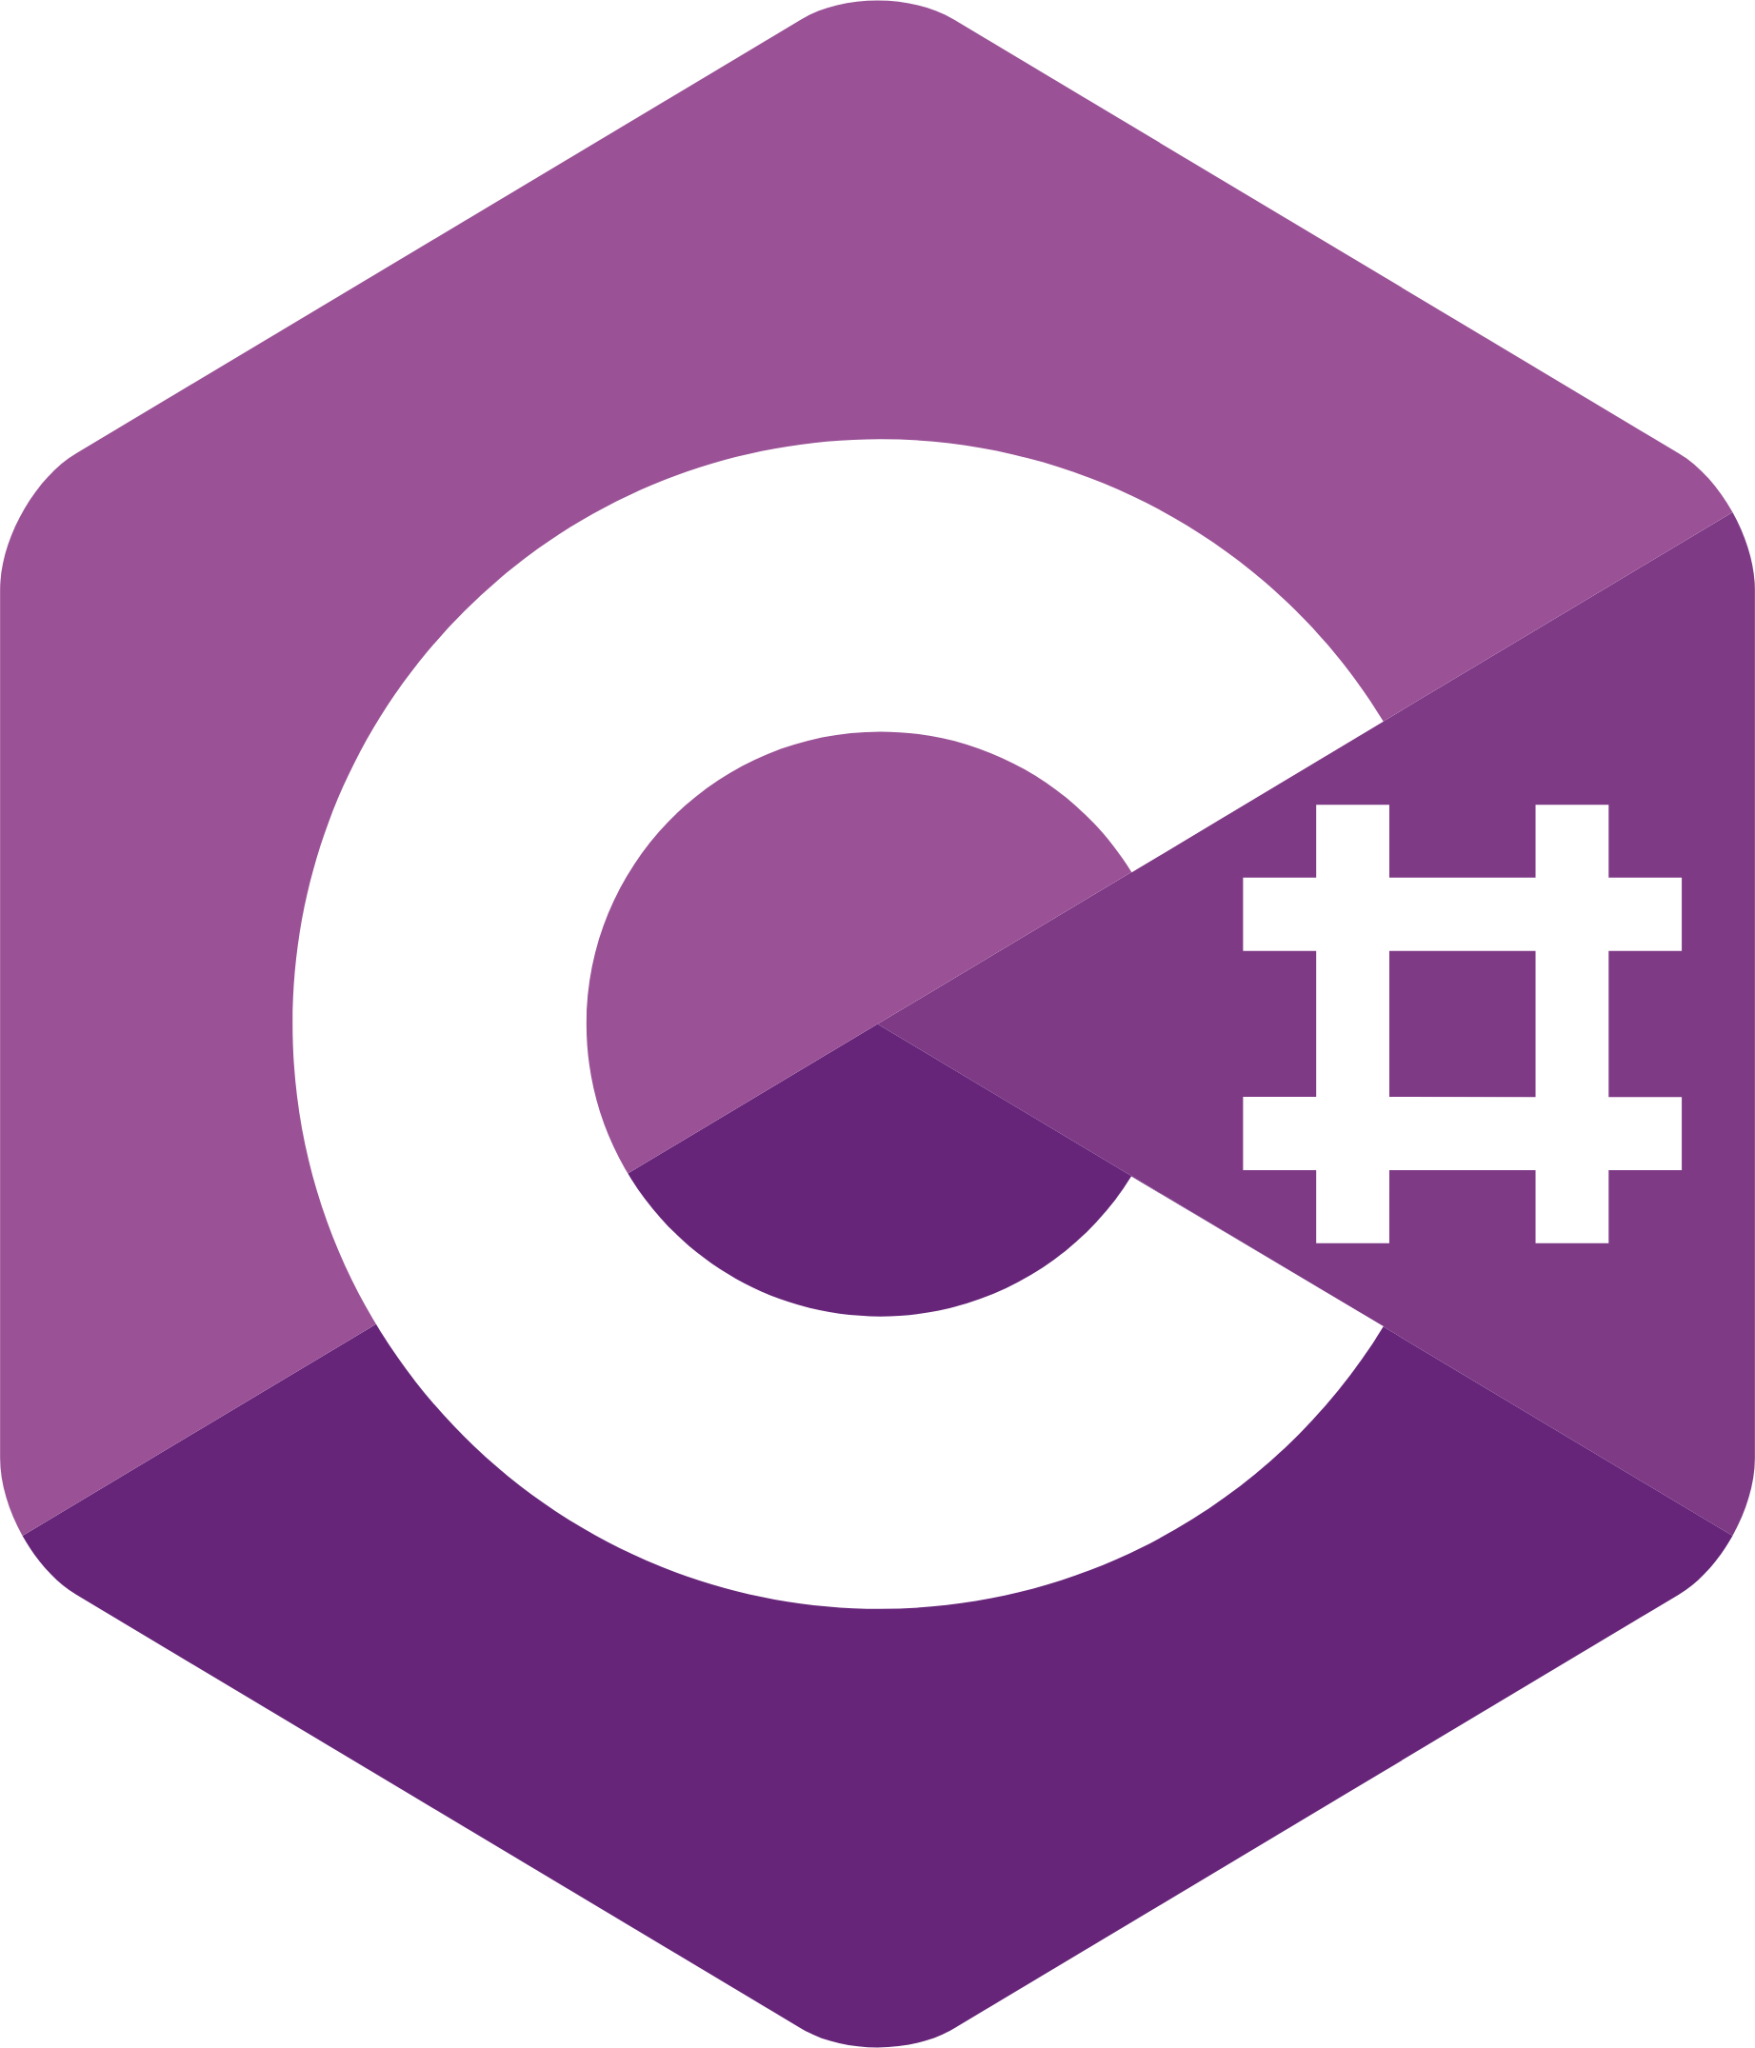
\includegraphics[width=0.25\textwidth]{chatbot/csharp-icon}
        \caption{Logo di C\#}
    \end{minipage}\hfill
    \begin{minipage}[t]{0.5\textwidth}
        \centering
        
\includegraphics[width=0.25\textwidth]{chatbot/dotnet-icon}
        \caption{Logo di .NET Core}
    \end{minipage}
\end{figure}

\section{Architettura}

Il ChatBot si compone di due parti principali: il \emph{Bot} vero e proprio e il l'\emph{HttpListener} (o \emph{WebServer}). 
Il primo è responsabile dell'autenticazione del \emph{Bot} e della gestione delle \emph{chat} con gli utenti, mentre il secondo si occupa della ricezione delle notifiche tramite \emph{HTTP}.

Il \emph{Bot} è in grado di creare nuove conversazionu, inviare nuovi messaggi e creare \emph{subscription}.

Una \emph{subscription} è un meccanismo che permette di ricevere notifiche in tempo reale da un servizio \emph{API}, in questo caso da Microsoft Teams attraverso il servizio \emph{Graph API}.
Per creare una \emph{subscription} è necessario specificare l'\emph{endpoint}\footnote{Un endpoint è un URL che rappresenta una specifica risorsa o funzionalità in un'API. Gli endpoint consentono ai client di interagire con i server tramite HTTP(S)} a cui inviare le notifiche, il tipo di evento da monitorare e il \emph{certificato} per la cifratura delle notifiche.

L'\emph{HttpListener} si occupa della gestione delle notifiche generate dalle \emph{subscription}, validando i dati ricevuti e inviando le informazioni al \emph{Bot}.


\section{Utilizzo di token e crittografia}

I token \emph{JWT} sono stati utilizzati in due casi per il funzionamento del \emph{ChatBot}:
\begin{itemize}
	\item Per l'autenticazione del \emph{Bot} con il servizio \emph{Graph API} di Microsoft.
	\item Per la verifica dell'autenticità delle notifiche inviate dal servizio \emph{Graph API} al \emph{WebServer}.
\end{itemize}

Il primo caso viene gestito automaticamente dalla libreria \emph{Microsoft.Graph} che si occupa di generare e rinnovare i token necessari per l'autenticazione.
Questo processo è trasparente all'utente e non richiede alcuna configurazione aggiuntiva.

Il secondo caso, invece, è gestito manualmente, verificando la firma del token ricevuto dal servizio \emph{Graph API}.
Inoltre il contenuto delle notifiche viene crittografato con un \emph{certificato \gls{X.509}} per garantire la riservatezza delle informazioni.

\subsection{Creazione dei certificati}

\noindent La creazione dei \emph{certificati} avviene tramite il seguente codice:

\lstset{
    language=[Sharp]C,
    basicstyle=\ttfamily,
    keywordstyle=\color{blue},
    stringstyle=\color{red},
    commentstyle=\color{green},
    tabsize=2,
    numbers=left,
    numberstyle=\color{gray},
    breaklines=true,
    captionpos=b,
    frame=single,
    showspaces=false,
    showstringspaces=false,
    breakatwhitespace=true,
    columns=fullflexible,
}

\begin{lstlisting}
	using RSA rsa = RSA.Create(2048);

	CertificateRequest request =
		new(
			"cn=NotificationServiceCertificate",
			rsa,
			HashAlgorithmName.SHA256,
			RSASignaturePadding.Pkcs1
		);

	using X509Certificate2 cert = request.CreateSelfSigned(
		DateTimeOffset.Now,
		DateTimeOffset.Now.AddYears(5)
	);

	string certificateBase64String = Convert.ToBase64String(
		cert.Export(X509ContentType.Cert)
	);

	CertificateConfig newCertificate =
		new()
		{
			CERTIFICATE_ID = Certificates.GetUniqueId(),
			CERTIFICATE = certificateBase64String,
			PRIVATE_KEY = Convert.ToBase64String(rsa.ExportRSAPrivateKey())
		};
\end{lstlisting}

Si può notare che i certificati vengono creati da \emph{RSA} a 2048 bit e vengono firmati con l'algoritmo \emph{SHA-256} utilizzando il padding dello standard \emph{PKCS\#1} (\emph{RS256})
Poiché viene inviata solo la chiave pubblica tramite il \emph{certificato}, la chiave privata può essere utilizzata per creare una firma digitale.
Questa firma può essere verificata da chiunque riceva il \emph{certificato}, in quanto esso contiene la chiave pubblica necessaria per la verifica.

Il \emph{certificato} viene quindi convertito a stringa \emph{Base64} e salvato localmente con la chiave privata e un identificativo univoco.

Il \emph{certificato} viene quindi inviato al servizio \emph{Graph API} per la creazione della \emph{subscription}, in modo che ogni sua notifica venga crittografata con la chiave pubblica.

\subsection{Validazione delle notifiche}

Ogni notifica ricevuta deve essere validata seguendo certi passaggi che garantiscono l'autenticità del mittente e la riservatezza delle informazioni.

Il primo passo è la validazione dei token \emph{JWT}. 
\begin{enumerate}
	\item Il token non deve essere scaduto.
	\item È necessario poi verificare che il token non sia stato manomesso e che sia stato rilasciato da Microsoft ottenendo la chiave pubblica dall'\emph{endpoint} specificato nella documentazione\footcite{site:rich-notification}.
	\item Infine, è necessario verificare che il token sia stato rilasciato per la propria applicazione. Questo passaggio viene effettuato verificando che il campo \emph{audience} del token sia uguale all'\emph{AppId} dell'applicazione.
\end{enumerate}

\noindent La libreria \emph{Microsoft.IdentityModel.Tokens} fornisce un aiuto per la validazione dei token.

\begin{lstlisting}
	private static async Task<bool> ValidateJWTToken(string token, IEnumerable<string> appIds)
	{
		ConfigurationManager<OpenIdConnectConfiguration> configurationManager =
			new(
				"https://login.microsoftonline.com/common/v2.0/.well-known/
				openid-configuration",
				new OpenIdConnectConfigurationRetriever()
			);

		OpenIdConnectConfiguration openIdConfig =
			await configurationManager.GetConfigurationAsync();
		JwtSecurityTokenHandler handler = new();

		try
		{
			handler.ValidateToken(
				token,
				new TokenValidationParameters
				{
					ValidateIssuer = true,
					ValidateAudience = true,
					ValidateIssuerSigningKey = true,
					ValidateLifetime = true,
					ValidIssuer =
						$"https://login.microsoftonline.com/
						{ConfigManager.ConfigManager.Config.TENANT_ID}/v2.0",
					ValidAudiences = appIds,
					IssuerSigningKeys = openIdConfig.SigningKeys
				},
				out _
			);

			return true;
		}
		catch (Exception ex)
		{
			Logger.Logger.LogError(ex, "Error validating JWT token");
		}

		return false;
	}
\end{lstlisting}